\documentclass[11pt,a4paper,openany,oneside,parskip=half*]{article}

\usepackage[utf8]{inputenc}
\usepackage{tocloft}
\usepackage{nomencl}
\usepackage{pdfpages}
\usepackage{scrextend}
\usepackage{bm}
\usepackage{cite}
\usepackage{amsmath}
\usepackage{graphicx}
\usepackage[justification=centering]{caption}
\usepackage{float}
\usepackage{multicol}
\usepackage{float}
\usepackage[section]{placeins}
\usepackage[english]{babel} 
\usepackage{geometry} %Gr�ߟe des Bodys innerhalb der Seite 
\usepackage[utf8]{inputenc} 
\usepackage{ifthen}

%bindet die benutzten Packages ein

\linespread{1.25}

\RequirePackage{ifthen}
\renewcommand{\nomgroup}[1]{%
  \ifthenelse{\equal{#1}{R}}{\item[\textbf{Roman Letters}]}{%
    \ifthenelse{\equal{#1}{G}}{\item[\textbf{Greek Letters}]}{%
      \ifthenelse{\equal{#1}{O}}{\item[\textbf{Operators}]}{}}}}

\renewcommand*\vec[1]{\boldsymbol{#1}}
\renewcommand*\matrix[1]{\boldsymbol{#1}}

%setzt die fettgedruckte Schreibweise fuer Vektoren und Matrizen

\geometry{top=3cm, bottom=4cm}
\geometry{bindingoffset=1.5cm} %offset zum binden
\newcommand{\HRule}{\rule{\linewidth}{0.5mm}}  % definere gerade Linie mit 0.5mm Dicke

\begin{document}
\begin{titlepage}
\begin{figure}[htp]
\vspace*{-3cm} 
\hspace*{2.7cm}  

\includegraphics{./Titelseite/rwth_aia_en_rgb.eps}
\end{figure}
\begin{center}
\textbf{Diese Arbeit wurde vorgelegt am Aerodynamischen Institut}
\end{center}
\begin{center} % ab hier zentriert
\vspace*{4.2cm} %lasse 4.5 cm Platz von oben
{ \huge \bfseries Investigations on two-way coupling effects of particle-laden decaying isotropic turbulent flows}\\[0.3cm] % Groߟe Buchstaben, fett gedruckt, lasse 0.3cm Platz nach unten
\HRule \\[0.5cm] %Linie, 0,5cm Platz nach unten
\textsc{\Large{Projektarbeit}}\\ %in Kapitälchen
\textsc{\Large{von}}\\
\textsc{\LARGE{Julian Stemmermann, Steffen Trienekens und Christian Soika}}\\[0.5cm]
\HRule \\[0.4cm]
{\Large{Aerodynamisches Institut der RWTH Aachen}}\\[.5cm]
{\large \today} \\[1.5cm] % heutiges Datum
\vfill % So viel Platz lassen, dass es bis zur Ende der Seite geht, wobei die Abstände bei dem nächsten vfill gleich sind
\begin{flushleft} \large  %Einrückung, groß
\begin{tabular}{ll} % Tabelle
Betreuer: &Konstantin Fr\"ohlich \\
Erstpr\"ufer: &Univ.-Prof.\,Dr.-Ing. Wolfgang Schr\"oder
\end{tabular}
\end{flushleft}
\vfill % So viel Platz lassen, dass es bis zur Ende der Seite geht
\end{center}
\end{titlepage}

\numberwithin{equation}{section} %bestimmt die Nummerierung der Gleichungen, in diesem Fall nach Kapitel anstatt sie einfach durchzunummerieren

\makenomenclature %erstellt und druckt die Nomenklatur-Tabelle

\renewcommand{\refname}{}
\renewcommand{\nomname}{}



\setlength{\columnsep}{30pt}
\setlength{\parindent}{0pt}

\pagebreak

\tableofcontents{} %erstellt die Inhaltsangabe
 
\pagebreak

\section{Nomenclature}
\printnomenclature
\pagebreak
\section{Introduction}
\begin{figure}[h]
	\centering
  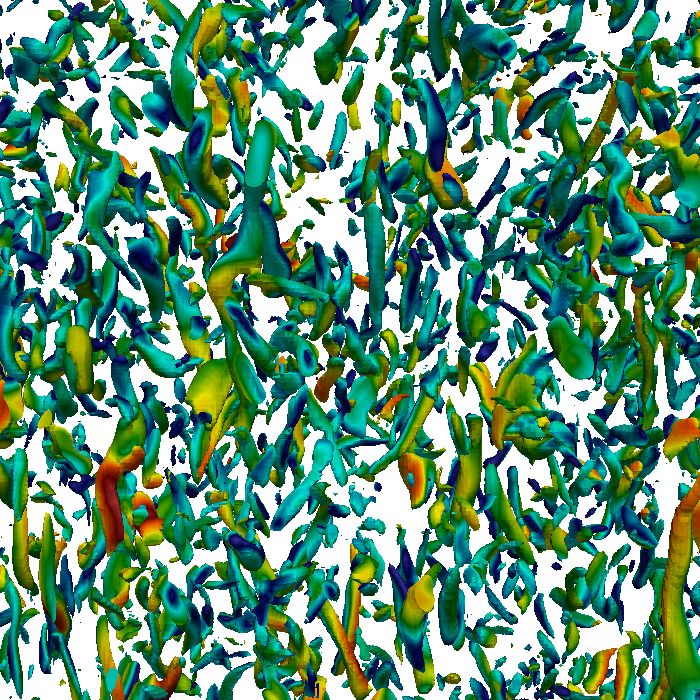
\includegraphics[width=\textwidth]{./Abbildungen/256_velocity_4.png}
	\caption{$\lambda_\mathrm{2}$-contours colored by velocity magnitude: Tubular structures in an isotropic flow field}
	\label{introuction_picture}
\end{figure}
This work deals with the effects of particles on an the flow conditions of isotropic turbulent flows.
There are many examples of these particle laden turbulent flows in nature, for example in volcanic eruptions and in the "white water" of breaking waves.
\newline
Multiphase flows also occur in many technical applications. Spray automization in fuel injectors, cyclonic particle separation in oil refineries and sediment accumulation in pipelines are just three of many cases, where it is of huge interest to predict the influence of particles on the turbulence of the mean flow.
Of major industrial interest is the fuel dispersion and combustion in an petrol-powered engine. To get a homogeneous and fast combustion, both should take place at turbulent flow conditions. One could say it is an important question, in which way and intensity the particles influence the turbulence.
\newline
Another important example is an fluidized bed. This is an application to realize an effective suspension and combustion of fluid particles in a vessel. The particles, which are at the bottom of the vessel, are suspended by a fluid, in most cases a gas, that streams from beyond the particles threw the porous bottom, if the pressure is larger than the gravity of the particles. While this happens the fluid suspends the particles and the contact between fluid and particles is very intimate, which facilitates for example the combustion of material with a low caloric content, the in situ absorption of the pollutants deriving from the combustion and the action of a catalyst. This process aims to produce a suspension with less heterogeneous regions, what means bubbles with a much smaller concentration of particles. Hence turbulence is very important requirement to produce a homogeneous fluid stream for effective and complete combustion.
\newline
In this work the influence of the particles on the streaming conditions is presented by using DNS and LES simulations. The focus lies on analyzing the energy transfer between particles and fluid as well as the intensity of the decrease of turbulent kinetic energy in the fluid.  
At the beginning some mathematical background information about modeling turbulent single phase and particle laden flows are given. 
Following the Navier-Stokes equations and the different scales of turbulent motion are presented as an approach to modelling turbulence. In addition to this for particle laden flows the equations of motion are expanded by a new term that describes the forces acting between fluid and particles. 
Also the coupling rate, that describes the exchanged energy is introduced.
Then the computational basics of methods used in this work are introduced. First the simulation methods DNS and LES, how they work and in which case which one is used is explained.
Them the used discretization tool to integrate the particle tracking equations, that works with a predictor-corrector-scheme, is described.     
Finally the computational method 'particle clustering' is introduced. This approach aims to decrease the computational effort of particle laden simulations. It works that way that the particles are coupled to cluster and each cluster is considered as one particle.
\newline
In the following the deviations caused by using this method are determined and the applicability is evaluated. Therefore the influence of the number of particles per cluster on the accuracy of the plots of the turbulent kinetic energy and the exchanged energy between particles and fluid per time is identified.
Also the number of particles that is needed to get consistent average values for the flow characteristics is investigated.
\pagebreak
\section{Mathematical models}
\subsection{Single-phase flow} %Christian
In this section the mathematical basics for understanding and simulating turbulent flows are discussed. However, it should be pointed out that this is no
complete treatise of the mathematical and physical basics. The reader can achieve further insight on this topic by looking at different books and papers, 
e.g. \cite{turbulentFlows}.
\newline
\subsubsection{The Navier-Stokes equations}
The Navier-Stokes equations are of great importance for understanding turbulent phenomena. This set of equations exists in forms for compressible and
incompressible fluids. For an infinitesimal small volume element $ \mathrm{d} \tau $ and using the cartesian coordinate system, 
they can be written in the so-called 'divergence form':
\nomenclature[o]{$\vec\nabla$}{Nabla-operator} %Erstellt automatisch die Nomenclature-Liste
\nomenclature[rQ]{$\vec{Q}$}{Container for conserved variables in the Navier-Stokes equations}
\nomenclature[rH]{$\vec{H}$}{Container for fluctuating variables in the Navier-Stokes equations}
\begin{equation}
  \frac{\partial{\vec{Q}}}{\partial{t}} + \vec\nabla \vec{H} = 0.
\end{equation}
The vector $ \vec{Q} $ contains all the variables which are conserved, i.e. the density $ \rho $, 
the velocity $ \vec{u} $ and the specific inner energy $ E $: 
\nomenclature[gr]{$\rho$}{Density}
\nomenclature[ru]{$\vec{u}$}{Velocity}
\nomenclature[rE]{$E$}{Specific inner energy}
\begin{equation}
 \vec{Q}= \left( \begin{array}{c}\rho\\\rho \vec{u}\\\rho E \end{array} \right).
\end{equation}
$ \vec{H} $ is the flux vector which stores all the floating variables and may be split up into two parts:
\nomenclature[rHi]{$\vec{H^\mathrm{i}}$}{Stores the inviscid variables in the flux-vector included in the Navier-Stokes equations}
\nomenclature[rHv]{$\vec{H^\mathrm{v}}$}{Stores the viscous variables in the flux-vector included in the Navier-Stokes equations} 
\begin{equation}
 \vec{H} = \vec{H^\mathrm{i}} + \vec{H^\mathrm{v}}.
\end{equation}
The contents of the two vectors are displayed below:
\nomenclature[rp]{$p$}{Pressure}
\nomenclature[rRe]{$Re$}{Reynolds number}
\nomenclature[gt]{$\matrix{\tau}$}{Stress tensor}
\nomenclature[rq]{$\vec{q}$}{Heat conduction}
\begin{equation}
 \vec{H^\mathrm{i}} = \left( \begin{array}{c}\rho \vec{u}\\\rho \vec{u} \vec{u} + p\\\vec{u} (\rho E + p) \end{array} \right),
\end{equation}
\begin{equation}
 \vec{H^\mathrm{v}} = - \frac{1}{Re} \left( \begin{array}{c}\ 0 \\ \matrix{\tau}\\ \matrix{\tau} \vec{u} + \vec{q} \end{array} \right).
\end{equation}
$ \vec{H^\mathrm{i}} $ is called inviscid flux and contains only the variables that are independent of the fluids viscosity, it describes the way a fluid 
with a viscosity of zero would behave. In contrast, the viscous flux $ \vec{H^\mathrm{v}} $ represents the effects of viscosity. The Reynolds number 
$ Re = \frac{\rho v d}{\mu} $ is defined to be the ratio of inertia to tenacity, which makes it very valuable for understanding turbulent flows. This is also due to the 
fact that two familiar objects with the same Reynolds number behave similar in turbulence.
To solve the Navier-Stokes equations, more information regarding some variables is required. For Calculating the specific inner Energy $ E $ 
and the heat conduction $ \vec{q} $, the following equations are used:
\nomenclature[gg]{$\gamma$}{Isentropic exponent}
\nomenclature[re]{$e$}{Specific internal energy}
\nomenclature[rPr]{$Pr$}{Prandtl number}
\nomenclature[gm]{$\mu$}{Dynamic viscosity}
\begin{equation}
 E = e  \frac{1}{2} \vec{|u|}^2,
\end{equation}
\begin{equation}
 \vec{q} = - \frac{\mu}{Pr (\gamma - 1)} \vec\nabla T
\end{equation}
with 
\nomenclature[rcp]{$c_p$}{Specific isobaric heat capacity}
\nomenclature[rcv]{$c_v$}{Specific isochoric heat capacity}
\begin{equation}
 \gamma = \frac{c_p}{c_v}
\end{equation}
and the Prandtl number
\nomenclature[rkt]{$k_t$}{Thermal conductivity}
\begin{equation}
 Pr = \frac{\mu_\infty c_p}{k_t}
\end{equation}
using the specific heat capacities of the fluid $ c_v $ and $ c_p $.
If one could assume that the fluid is a newtonian fluid, the linear correlation between stress and the rate of strain results in:
\nomenclature[rI]{$\matrix{I}$}{Identity tensor}
\nomenclature[rS]{$\matrix{S}$}{Rate-of-strain-tensor}
\nomenclature[rT]{$T$}{Temperature}
\begin{equation}
 \matrix{\tau} = 2 \mu \matrix{S} - \frac{2}{3} \mu (\vec\nabla * \vec{u}) \matrix{I}
\end{equation}
in which $ \matrix{S} = \frac{(\vec\nabla \vec{u})(\vec\nabla \vec{u})^T}{2} $ denotes the rate-of-strain-tensor. Additionally, the viscosity
$ \mu $ can be approximated through Sutherland's law, which is based on the ideal gas-theory: 
\nomenclature[rS]{$S$}{Sutherland temperature}
\nomenclature[rR]{$R$}{Universal gas constant}
\begin{equation}
 \mu (T) = \mu_\infty \biggl(\frac{T}{t_\infty}\biggl)^{3/2} \frac{T_\infty + S}{T + S}.
\end{equation}
S is in this case the Sutherland temperature.
To achieve closure the caloric state equation $ e = c_v T $ and the state equation for an ideal gas $
p = \rho R T $ are used. The specific gas constant is determined by $ R = c_p - c_v $. 
These equations form a set of partial differential equations, as a consequence starting values are needed.
\pagebreak
\subsubsection{Turbulent motion across all scales}
Turbulent flows contain eddies of all sizes and forms. Large-scale eddies bring energy to the flow which is then passed down to smaller-scale eddies and in the end dissipated into heat by viscous effects. This behavior is called the 'energy cascade' and was first described by Richardson in the year 1920 \cite{Richardson1920}. The theory then was developed further by Kolmogorov and published 1941 \cite{Kolmogorov1941}.
\newline
The first set of scales describe the large eddies. These scales are called \textit{integral} scales and are determined by the physical boundaries of the flow. As said before, at these scales the energy is brought into the flow, creating the so-called 'energy-containing range'. The length scale is the called integral length scale $L$, and the corresponding timescale which is most times called 'eddy turnover time' is defined as:
\nomenclature[gtL]{$\tau_\mathrm{L}$}{Eddy turnover time}
\nomenclature[rL]{$L$}{Integral length scale}
\nomenclature[rU]{$U$}{Characteristic velocity}
\nomenclature[rt*]{$t^*$}{Eddy turnover time}
\begin{equation}
\tau_\mathrm{L} = \frac{L}{U},
\end{equation}
where $U$ denotes the characteristic velocity.
\newline
The smallest scales in a turbulent flow are the Kolmogorov length ($\eta$) and time ($\tau_\mathrm{\eta}$) scale. At this scales, the effects of viscosity take place and the energy dissipates into heat. With the estimate $\epsilon \sim \frac{U^3}{L} $ they can be written as
\nomenclature[gh]{$\eta$}{Kolmogorov length scale}
\nomenclature[gth]{$\tau_\mathrm{\eta}$}{Kolmogorov time scale}
\begin{equation}
\eta = \biggl (\frac{\nu^3 L}{U^3} \biggl )^{1/4},
\end{equation}
\begin{equation}
\tau_\mathrm{\eta} = \biggl (\frac{\nu L}{U^3} \biggl ).
\end{equation}
Both these scales are coupled by the Reynolds number:
\begin{equation}
\frac{L}{\eta} = Re^{3/4},
\end{equation}
\begin{equation}
\frac{\tau_\mathrm{L}}{\tau_\mathrm{\eta}} = {Re_\mathrm{L}}^{1/2}.
\end{equation}
It can be seen from these to equations that the spacing between the scales increases for higher Reynolds numbers. 
\newline
A scale between these two is the Taylor microscale, often referred to as 'turbulence length scale'. 
\nomenclature[gl]{$\lambda$}{Taylor microscale}
Although it lacks of a physical interpretation, it is often used to describe the intermediate range between integral and Kolmogorov scales. 
This scales definition is: 
\begin{equation}
\lambda = \sqrt{15 \frac{\nu}{\epsilon}} |\vec{v'}|
\end{equation}
with $|\vec{v'}|$ denoting the absolute value of the velocities fluctuation. This scale can be used to compute another Reynolds number $Re_\mathrm{\lambda}$:
\begin{equation}
Re_\mathrm{\lambda} = \frac{|\vec{v'}| \lambda}{\nu}.
\end{equation}
Together these scales form a powerful tool to understand, compute and describe turbulent flows. 
\pagebreak
\subsection{Particle dynamics} %Steffen
\textbf{Gravity anschauen, Terminal Velocity einfuegen}
\newline
This work deals with particle laden fluids, therefore the impact of them on the flow behavior of the fluid needs to be described. The phenomenon described in this script is called two-way-coupling. This chapter is based on \cite{computationalMethodsforMultiphaseFlow}.
\newline
In this context small and heavy rigid particles with a spherical shape are considered. The basic equation of motion for this case is the Maxey Riley equation that can be achieved from \cite{EquationOfMotionForASmallRigidSphereInANonuniformFlow}. Their radius $ r_p $ is even smaller than the Kolmogorov scale $ \eta $, but also large enough to neglect the Brownian motion.
\newline
Due to the \textbf{small particle concentration}, the best and most common way to describe these flows is the point particle approach, which means that every particle is treated as a mathematical point source of mass, momentum and energy. In this case the focus lies on the momentum exchange, effects like particle-particle interactions and particle-wall interactions are neglected.  
\newline
At describing the motion of the particles in the following the fact that we deal with gas-solid flows is an advantage, since several simplifications can be made.
\newline
First the perspective is taken on the influence of the particles on the carrier fluid. Here the assumptions that the fluid is incompressible and that there is no mass exchange over the particle surface are used. In addition to this the gravity is neglected in the used simulations.
Hence the continuity equation becomes
\begin{equation}
\vec{\nabla} \cdot\vec{u} = 0.
\end{equation}
After including all the simplifications mentioned before the Navier-Stokes equations - described in chapter 1 - become
\begin{equation}
\rho\biggl(\frac{\partial{\vec{u}}}{\partial{t}}+\vec{\nabla} \cdot (\vec{u}\vec{u})\biggl) = -\vec{\nabla}p + \mu\nabla^\mathrm{2}\vec{u}-\vec{F}.
\end{equation}
\nomenclature[rF]{$\vec{F}$}{Force per unit volume from particle on fluid}
The influence of the particles on the fluid is represented by the new term $\vec{F}$, wich describes the force per unit volume on the fluid.
$\vec{F}$ could be approximated by a superposition of Dirac's delta functions over all particles, centered at the location $x_p^n$ of each particle:
\nomenclature[rfn]{$\vec{f}^\mathrm{n}$}{Sum of forces acting on the fluid}
\begin{equation}
\vec{F} = \sum \limits_{n=1}^{N_\mathrm{p}} \vec{f}^\mathrm{n}(\vec{x}_\mathrm{p}^\mathrm{n})\delta(\vec{x}-\vec{x}_\mathrm{p}^\mathrm{n}).
\end{equation}
$\vec{x}_\mathrm{p}^\mathrm{n} $ is the position of the n-th particle and results from the kinematic equation 
\begin{equation}
 \frac{\mathrm{d}\vec{x}_\mathrm{p}}{\mathrm{d}t} = \vec{v}_\mathrm{p}^\mathrm{n},
\end{equation}
with $\vec{v}_{\mathrm{p}}^\mathrm{n}$ being the velocity of the n-th particle.
\newline
$\vec{f}^\mathrm{n}$ is the sum of forces acting between fluid an particles. The delta function results in one if $\vec{x}-\vec{x}_\mathrm{p}^\mathrm{n}$ becomes zero and otherwise it is zero. By this means, the coupling forces act at the position of each particle on the fluid. 
\newline
Also it plays an important role in the equation of motion of the particles:
\begin{equation}
\mathrm{v}_\mathrm{p} \rho_\mathrm{p} \frac{\mathrm{d}\vec{v}_\mathrm{p}^\mathrm{n}}{\mathrm{d}t} = \mathrm{v}_\mathrm{p} \rho_\mathrm{p}+\vec{f}^\mathrm{n}(\vec{x}_\mathrm{p}^\mathrm{n})
\end{equation}
\nomenclature[rv]{$\mathrm{v}_\mathrm{p}$}{Particle volume}
As already mentioned $\vec{f}^\mathrm{n}(\vec{x}_\mathrm{p}^\mathrm{n})$ could be divided in several forces. Then the equation of particle motion looks like:
\begin{equation} \label{navier_stokes_particle}
m_\mathrm{p} \frac{\mathrm{d}\vec{v}_\mathrm{p}^\mathrm{n}}{\mathrm{d}t} = m_\mathrm{p}+\rho \mathrm{v}_\mathrm{p}\biggl(\frac{\mathrm{D}\vec{u}}{\mathrm{D}t}- \biggl)+\vec{f}_\mathrm{d}+\vec{f}_\mathrm{l}+\vec{f}_\mathrm{a}+\vec{f}_\mathrm{h}+\vec{f}_\mathrm{additional}
\end{equation}
\nomenclature[rfd]{$\vec{f}_\mathrm{d}$}{Drag force}
\nomenclature[rfl]{$\vec{f}_\mathrm{l}$}{Lift force}
\nomenclature[rfa]{$\vec{f}_\mathrm{a}$}{Added mass force}
\nomenclature[rfh]{$\vec{f}_\mathrm{h}$}{History force}
\nomenclature[rRep]{$Re_\mathrm{p}$}{Particle Reynolds number}
Here $\vec{f}_\mathrm{d}$ represents the hydrodynamical drag force that is parallel to the undisturbed streamlines, which depends on an empirical drag coefficient $C_{\mathrm{d}} $:
\begin{equation}
\vec{f}_\mathrm{d}=-\frac{3}{4}\rho \mathrm{v}_\mathrm{p} \frac{C_\mathrm{d}}{d_\mathrm{p}}|\vec{v}_\mathrm{p}-\vec{u}|(\vec{v}_\mathrm{p}-\vec{u})
\end{equation}
It depends on the empirical drag coefficient defined after Schiller and Naumann as
\begin{equation} \label{C_d}
C_\mathrm{d} = \frac{24}{Re_\mathrm{p}}(1+0.15Re_\mathrm{p}^\mathrm{0.687}).
\end{equation}
$\vec{u}$ is the velocity of the uniform stream, which is distant enough from the particle that it is not disturbed by it.
The other partial hydrodynamical force, the lift force $\vec{f}_\mathrm{l}$ is perpendicular to the undisturbed streamlines.
Furthermore the added mass force $\vec{f}_\mathrm{a}$ represents the influence of the fluid's inertia that has an impact on the particle, if it has a different acceleration than the mean flow.
Hence it could be determined by
\begin{equation}
\vec{f}_\mathrm{a} =  \frac{1}{2}\rho \mathrm{v}_\mathrm{p} \biggl(\frac{\mathrm{D}\vec{u}}{\mathrm{D}t}-\frac{\mathrm{d}\vec{v}_\mathrm{p}}{\mathrm{d}t}\biggl)
\end{equation}
The history force $\vec{f}_\mathrm{h}$ takes diffusion and convection that results from of the vortices behind the particles into account. Basselt's result, neglecting the finite size correction, is proportional to $\vec\nabla^\mathrm{2}\vec{u}$:
\begin{equation}
\vec{f}_\mathrm{h} = \frac{3}{2}d_\mathrm{p}^\mathrm{2}\rho\sqrt{\pi\nu}\int_{t_\mathrm{0}}^{t} \frac{\mathrm{d}t'}{(t-t')^\mathrm{1/2}} \biggl(\frac{\mathrm{D}\vec{u}}{\mathrm{D}t'}- \frac{\mathrm{d}\vec{v}_\mathrm{p}}{\mathrm{d}t'}\biggl).  
\end{equation}
\nomenclature[gn]{$\nu$}{Kinematic viscosity}
The last term $\vec{f}_\mathrm{additional}$ is attached for the case that we have to take other forces like electrostatic interactions into account.
In this case of gas-solid suspensions several simplifications could be made.
\newline
In the following the fact that the added mass force, the lift force and the history force are negligible small compared to the drag force is shown using a rough approximation.
Vincenzo Armenio and Virgilio Fiorotto \cite{TheImportanceOfTheForcesActingOnParticlesInTurbulentFlows} show that the added mass force is much smaller than the drag force for all density ratios and that ratios among the forces and the Stokes drag decrease with rising particle density.
The relation of the history force and the added mass force with the assumption of comparable accelerations, with the relaxation time of the order of $\tau$ results in
\begin{equation}
\frac{|\vec{f}_\mathrm{h}|}{|\vec{f}_\mathrm{a}|}\simeq 18 \sqrt{\frac{\nu\tau}{d_\mathrm{p}^\mathrm{2}}}.
\end{equation}
\nomenclature[rd]{$d_\mathrm{p}$}{Particle diameter}
Hence it is of the order of the ratio of the diffusion length to the particle diameter, which might be of the order of one, if $\tau \sim \frac{d_\mathrm{p}^\mathrm{2}}{\nu}$.
\nomenclature[gtp]{$\tau_\mathrm{p}$}{Particle relaxation time}
It follows that the history force is also negligible compared to the drag force.
For the lift force the situation is similar, because is is also proportional to the fluid density and the length scale of the ambient flow vorticity might be much greater than the particle size.
It shows that the particle motion is only depending on the the hydrodynamical drag force which results from the actual difference between the fluid velocity $\vec{u}(\vec{x}_\mathrm{p})$ at particle position $\vec{x}_\mathrm{p}$ and the particle velocity $\vec{v}_\mathrm{p}$.
Due to this assumptions (\ref{navier_stokes_particle}) becomes
\begin{equation}
\rho_\mathrm{p}\frac{\mathrm{d}\vec{v}_\mathrm{p}^\mathrm{n}}{\mathrm{d}t} = \rho_\mathrm{p}+\vec{f}_\mathrm{d}^\mathrm{n}.
\end{equation}
This equation can be rewritten with help of the relaxation time $\tau_\mathrm{p}$, which physically represents the time scale over which the drag force decreases the particle's relative velocity to zero. At one point in the fluid with the proportionality 
\begin{equation}
\frac{\rho_\mathrm{p} v_\mathrm{p}}{\tau_\mathrm{p}^\mathrm{n}} \sim f_\mathrm{d}
\end{equation} 
it follows the equation for the relaxation time
\begin{equation}
\tau_\mathrm{p}^\mathrm{n} = \frac{4}{3}\frac{\rho_\mathrm{p}}{\rho} \frac{d_\mathrm{p}}{C_\mathrm{d}^\mathrm{n}}\frac{1}{v_\mathrm{r}^\mathrm{n}},
\end{equation}
where $v_\mathrm{r}^\mathrm{n}$ is the relative velocity. 
With equation (\ref{C_d}) and the Reynolds number in relation to the particles $Re_\mathrm{p}^\mathrm{n}=\frac{v_\mathrm{r}^\mathrm{n}d_\mathrm{p}}{\nu}$, with the particle diameter $d_\mathrm{p}$ it follows:
\begin{equation}
\tau_\mathrm{p}^\mathrm{n} = \frac{\rho_\mathrm{p}}{p}\frac{d_\mathrm{p}^2}{18\nu}\frac{1}{1+0.15Re_\mathrm{p}^\mathrm{n^\mathrm{0.687}}}.
\end{equation} 
Then the equation of motion of the particles becomes
\begin{equation}
\rho_\mathrm{p}\frac{\mathrm{d}\vec{v}_\mathrm{p}^\mathrm{n}}{\mathrm{d}t} = \rho_\mathrm{p}-\rho_\mathrm{p}\frac{\vec{v}_\mathrm{p}^\mathrm{n}-\vec{u}^\mathrm{n}}{\tau_\mathrm{p}^\mathrm{n}}.
\end{equation}
Using the Stokes response time $\tau_\mathrm{ps} =\frac{d^2}{18 \nu} \frac{\rho_\mathrm{p}}{\rho}$, that is the particle response time at resting fluid conditions, there finally exists another form of this equation 
\nomenclature[gtps]{$\tau_\mathrm{ps}$}{Stokes relaxation time}
\begin{equation}
\rho_\mathrm{p}\frac{\mathrm{d}\vec{v}_\mathrm{p}^\mathrm{n}}{\mathrm{d}t} = \rho_\mathrm{p}-\rho_\mathrm{p}\frac{\vec{v}_\mathrm{p}^\mathrm{n}-\vec{u}^\mathrm{n}}{\tau_\mathrm{ps}}f_\mathrm{d},
\end{equation}
with $f_\mathrm{d} = 1+0.15Re_\mathrm{p}^\mathrm{n^{0.687}}$, which is a correction factor describing the flow conditions and not the drag force mentioned before.
\newline
\nomenclature[rrp]{$r_\mathrm{p}$}{Particle radius}
\nomenclature[grp]{$\rho_\mathrm{p}$}{Particle density}
\nomenclature[rxp]{$\vec{x}_\mathrm{p}$}{Particle position}
\nomenclature[rvp]{$\vec{v}_\mathrm{p}$}{Particle velocity}
\nomenclature[rD]{$f_\mathrm{D}$}{Drag correction}
The coupling rate $\psi$, that describes the transferred Energy per time between particles and fluid, is defined as
\begin{equation}
\psi = \vec{F} \vec{u}. 
\end{equation}
\nomenclature[gx]{$\psi$}{Coupling rate}
Hence it results from the force per unit volume exerted between the fluid and the particles and the main velocity of the fluid.
It is an useful variable to describe how much the main fluid and the particles influence each other.
\pagebreak
\section{Numerical methods} %Julian
To simulate flows like those described above there are two options. The direct numerical simulation (DNS) is the easier one to understand, although it is numerically very expensive. The Large-eddy simulation (LES) is numerically more capable, still we must accept certain inaccuracies. These two numerical methods are now discussed in the following chapter.
\subsection{Direct numerical simulation}
The basis of the direct numerical simulation (DNS) are the Navier-Stokes equations as described above. The idea is that the computer is very good at calculating and solves these equations completely. This provides a very accurate result, as all scales of motion are being resolved. Still it requires an immense level of computational resources which increases rapidly with the Reynolds number. These computational resources were not available until the 1970s. Even though it is not advisable to resolve every scale of motion, if only the contained energy is of greatest interest. With the large-eddy simulation, as described below, the computational effort is 99.98 \% less compared to DNS, which indeed is the fraction of the dissipative scale. This leaves 0.02 \% of the flow, which is correlative with the fraction of the energy-containing larger-scale \cite{turbulentFlows}.%zum Uebergang zu LES siehe Pope S. 352 und Fig. 9.4
\subsection{Large-eddy simulation}
Due to the fact that DNS is effortful and wasting resources if a fully resolved resolution is not required, large-eddy simulation (LES) was created to save time and resources. This is especially efficient if mainly the temporal energy trend is considered, because the energy containing larger-scale motion is completely resolved and the indeed small effects of the expensive smaller-scale motion are just modeled. Otherwise in DNS resolving the small dissipative scale would require most of the computational resources.
\newline
Simulating only the larger-scale motions is called filtering, which means that the smaller-scale motions, also known as fluctuation, are filtered out. For further information on filter functions, the works of Pope \cite{turbulentFlows} should be considered. To model the filtered smaller-scale motions usually a subgrid-scale (SGS) model is used. According to Hickel (2007) the interference between explicit SGS and the truncation error can be exploited, i.e. the truncation error can serve as model of the effects of unresolved scales, which is therefore an implicit SGS model. Thus we call it implicit LES (ILES) \cite{implicitLES}. %als Zitat die Dissertation TUM Hickel
\subsection{Discretisation}
To integrate the Lagrangian particle tracking equations, discussed above, a predictor-corrector scheme based on the trapezoidal rule for numerical integration
\begin{equation}
f (t + \delta t) \approx f(t) + \frac{\delta t}{2} \left[ \frac{\partial f(t)}{\partial t} + \frac{\partial f(t + \delta t)}{\partial t} \right ]
\end{equation}
is used.
\newline
The first step is the prediction of the new particle position $\vec{x}_{\mathrm{p}, n+1}$ using a Taylor expansion for a small time step $\delta t$
\begin{equation}
\vec{x}_{\mathrm{p}, n+1} = \vec{x}_{\mathrm{p}, n} + \delta t \vec{v}_{\mathrm{p}, n} + \frac{1}{2} \delta t^2 \vec{a}_{\mathrm{p}, n}.
\end{equation}
Due to the computational effort we will put the fluid velocity $\vec{u}(\vec{x}_{\mathrm{p}, n+1})$ at the particle position $\vec{x}_{\mathrm{p}, n+1}$ on the level of the nearest cell fluid velocity.
\newline
The updated velocity and acceleration are calculated as
\begin{equation}
\vec{v}_{\mathrm{p}, n+1} = \frac{\vec{v}_{\mathrm{p}, n} + \frac{1}{2} \delta t \left(\vec{a}_{\mathrm{p}, }n + \frac{f_\mathrm{D}}{\tau_\mathrm{p}}\vec{u}(\vec{x}_{\mathrm{p}, n+1}) \right)}{1 + \frac{1}{2} \frac{f_\mathrm{D}}{\tau_\mathrm{p}} \delta t},
\end{equation}
\begin{equation}
\vec{a}_{\mathrm{p}, n+1} = \frac{\frac{f_\mathrm{D}}{\tau_\mathrm{p}} \left(\vec{u}(\vec{x}_{\mathrm{p}, n+1}) - \vec{v}_{\mathrm{p}, n} - \frac{1}{2} \delta t \vec{a}_{\mathrm{p}, n} \right)}{1 + \frac{1}{2} \frac{f_\mathrm{D}}{\tau_\mathrm{p}} \delta t}.
\end{equation}
The updated particle position must be corrected by an additional term according to the trapezoidal rule
\begin{equation}
\vec{x}_{\mathrm{p}, n+1} = \vec{x}_{\mathrm{p}, n} + \frac{1}{2} \delta t \left( \vec{v}_{\mathrm{p}, n+1} + \vec{v}_{\mathrm{p}, n} \right) + \frac{1}{12} \delta t^2 \left( \vec{a}_{\mathrm{p}, n+1} - \vec{a}_{\mathrm{p}, n} \right).
\end{equation}
\subsection{Particle clustering}
\nomenclature[rmc]{$m_\mathrm{c}$}{Number of clustered particles}
The high number of point particles require even more computational resources for the particle-laden simulation. The main idea to reduce this requirement is to create clusters of point particles, meaning that a new variable $m_\mathrm{c}$ is introduced. We consider a cluster of $m_\mathrm{c}$ point particles as one larger point particle, i.e. the program has less particles to simulate. To compensate this lack of particles, the coupling force is multiplied by $m_\mathrm{c}$, due to the $m_\mathrm{c}$-fold mass of the (cluster-)particles. In chapter 5 (results) we evaluate the legitimacy of particle clustering and the maximum acceptable value of $m_\mathrm{c}$.
\newline
\newline
Projektion (noComputationalParticles), Diskretisierung
implizite LES (Motivation fuer LES -  Pope Chapter 9, Bild 9.4), DNS
\pagebreak
\section{Results}
The simulations were carried out using ZFS, the simulation tool developed and implemented at the Institute of Aerodynamics at RWTH Aachen University 
\cite{anAdaptiveMultilevelMultigridFormulationForCartesianHierarchicalGridMethods} \cite{aStrictlyConservativeCartesianCutCellMethodForCompressibleViscousFlowsOnAdaptiveGrids}. 
The tool is capable of simulating finite-volume flows of compressible fluids. In the simulations, which results the reader can see at hand, the Mach-number $Ma$ was set to 0.1 to simulate an almost incompressible fluid.
The turbulence was simulated on a cubic grid using $64^3$,$96^3$,$128^3$ and $256^3$ grid points. As a consequence of grid refinement the first three cases were simulated using LES, 
the case in which $256^3$ cells were used is carried out as DNS. Further information can be gained by looking at \cite[p.344-357 for DNS and p. 558-639 for LES]{turbulentFlows}.
\begin{figure}[h]
	\centering
  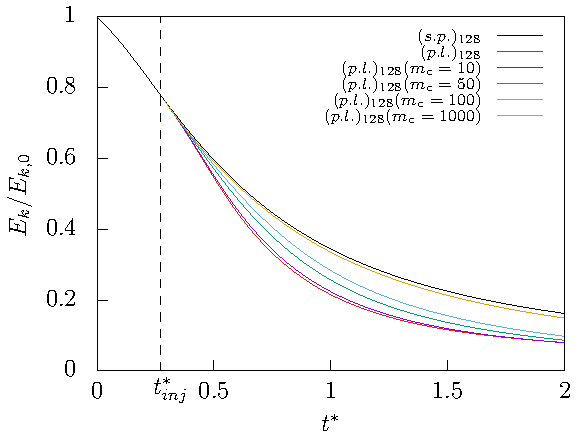
\includegraphics[width=0.9\textwidth]{./Abbildungen/128/kineticEnergy_time.pdf}
	\caption{Kinetic Energy over eddy turnover times for different numbers of clustered particles with fixed all-over particle number}
	\label{kineticEnergy_time_128}
\end{figure}
\newline
For simplification, the special case of isotropic turbulence was used. For this idealized flow form the statistical 
velocities are invariant in all directions of the grid. It follows that the flow velocity is also invariant for rotations and reflections. 
The turbulence was initialized using a seed-based random generator. To achieve physical results, the simulation of the particle-free flow was carried out a reasonable amount of time, 
at which a restart file was written out. This procedure ensures a fully developed turbulent 
flow, which has emancipated from the initialization. In this flow field, a specific number of spherical particles were injected. 
\newline
With the aim of minimized computational effort for simulating the particle-laden flow while still achieving high quality results, a clustering of particles was integrated into the simulation tool. To investigate the differences in accuracy for different particles sizes, the variable $m_\mathrm{c}$ was introduced to the code describing the number of particles in one cluster. The simulations were then set up with the overall same number of particles ($ 10^6 $), altering just the number of particles in one cluster. Then the simulations were carried out normally and result in the graphs  at hand(Figure \ref{kineticEnergy_time_128}, \ref{der(kineticEnergy)_time_128} and \ref{coupling_time_128}). 
It can be seen in figure \ref{kineticEnergy_time_128} that the decay in kinetic energy from the starting point depends highly on the number of clustered particles. The kinetic energy in the particle-laden cases drops more rapidly in the time-period after the injection than the particle-free case due to a higher dissipation rate induced by the particles. 
\begin{figure}[h]
    \centering
    \begin{minipage}{.5\textwidth}
        \centering
        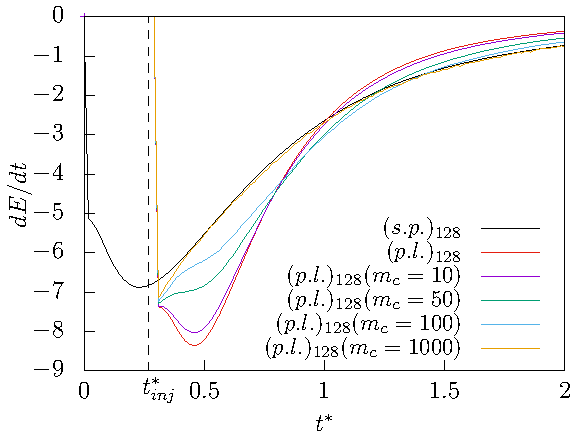
\includegraphics[width=\linewidth]{./Abbildungen/128/der(kineticEnergy)_time.pdf}
        \caption{Change in kinetic Energy over eddy turnover times}
        \label{der(kineticEnergy)_time_128}
    \end{minipage}%
    \begin{minipage}{0.5\textwidth}
        \centering
        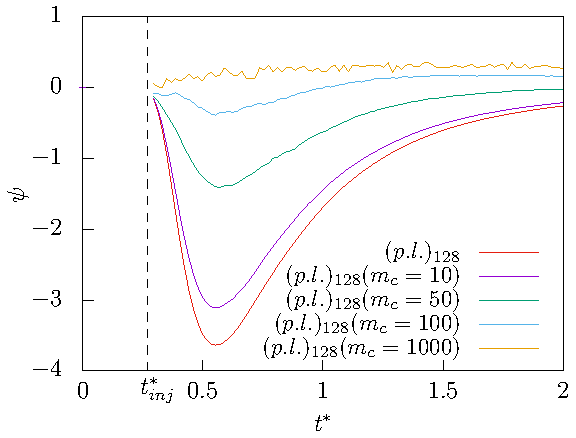
\includegraphics[width=\linewidth]{./Abbildungen/128/coupling_time.pdf}
        \caption{Coupling Rate over eddy turnover times}
        \label{coupling_time_128}
    \end{minipage}
\end{figure}
\newline
Fitting to this first results, the Graphs of figure \ref{der(kineticEnergy)_time_128} and \ref{coupling_time_128} clearly show that for simulations with highly clustered particles the results differ a lot from unclustered simulations. Looking at the results for the change in kinetic Energy, the difference becomes evident: The higher $ m_\mathrm{c} $ is, the lower is the drop in rate of change of the kinetic energy. It approaches more and more the particle free case. A similar result was found by Schneiders et al \cite{Schneiders2017}. The particles therefore have two effects on the fluid: Firstly, the viscous dissipation rises in the case of particle-load. Secondly, there is always an energy transfer from the particles to the surrounding fluid. Both of these effects influence the kinetic energy and an equality in the energy balance for the particles can be observed at about one eddy turnover time for the unclustered simulation. At this point in time the rate of kinetic energy flowing from the particles to the fluid matches the \textit{additional} rate of dissipated energy induced by the particles.
\newline
Schneiders` results show, that for particles with the same diameter this point is reached later in time for more dense particles due to their inertia. It could be observed a similar effect with the simulation at hand: The more particles are summarized in one cluster, the later the balanced state of energy flow an dissipation is achieved. From this point on, the kinetic energy drops slower than in the particle-free case.
\newline
In difference to the others, the case in which 1000 particles were clustered shows a strange behavior. It catches up to the particle-free case very fast, which leads to the conclusion that the amount of clusters is so small that the flow almost behaves like one without particles. Additionally the change in kinetic Energy shows inconstancy which can also be traced back to the small number of clusters. The amount is just to small to achieve high-quality information in the statistical variables. 
\newline
The same impression can be achieved by looking at the graphs describing the coupling rate (figure \ref{coupling_time_128}). The particle-laden-case makes the biggest jump into negative coupling rate. The higher the number of coupled particles, the lower is the amount of the coupling rate. This evolution continues until the physicality vanishes and the randomness starts to show at the results for $m_\mathrm{c}$ higher than 50. 
\newline
Being very similar in the time shortly after the injection, the flow statistics diverge more and more when time passes by. The variables of these simulations one turnover time after the injection can be found in table \ref{table_properties} on page \pageref{table_properties}. The ratio of the densities for this simulations was set to $\frac{\rho_\mathrm{p}}{\rho} = 1000$, the particle diameter was 0.0794048628, so that $d_\mathrm{p} \approx 0.6 \eta$. At the timestep of injection the Stokes response time $\tau_\mathrm{ps}$ was 0.03497, the Prandtl number was 0.72 and $Re_\lambda$ was 57.9757. In all of these simulations the volume and mass fractions $\phi_\mathrm{v}$ and $\phi_\mathrm{m}$ were constant ($\phi_\mathrm{v}= 10^{-3}$, $\phi_\mathrm{m}=1$).
\begin{table}[h]
\begin{center}
\begin{tabular}{l | c c c c c c c }
$m_\mathrm{c}$ & $\epsilon \frac{{u_0}^3}{L}$ & $\frac{\lambda}{L}$ & $\frac{\eta}{L} $ & $Re_\lambda$ \\
\hline
\hline
1 & 0.79150 & 0.0432 & 0.00333 & 43.360 &\\
10 & 1.02918 & 0.03866 & 0.00312 & 39.5653 &\\
50 & 1.78788 & 0.03144 & 0.00272 & 34.4702 &\\
100 & 2.26144 & 0.02940 & 0.00257 & 33.8869 &\\
1000 & 2.2855 & 0.03184 & 0.00256 & 39.8993 &\\
\hline
\end{tabular}
\caption{Variables of the first set of simulations one turnover time after injection for the $128^3$-case}
\label{table_properties}
\end{center}
\end{table}
\newline
To find out at which number of particles the results are sufficiently exact, a second set of simulations was carried out. As mathematics of turbulent flows are based on averaged variables, small numbers of particles can lead to false and even physically questionable results. In these simulations, no particle clustering was used, just different numbers of particles were injected into the same flow. For these simulations similar properties to the ones from the first set of simulations were used, just the mentioned number of particles was changed. An example for the deviation in kinetic energy for different numbers of particles can be found on page \pageref{kineticEnergy_numberOfParticles} on figure \ref{kineticEnergy_numberOfParticles}. 
\begin{figure}[h]
	\centering
  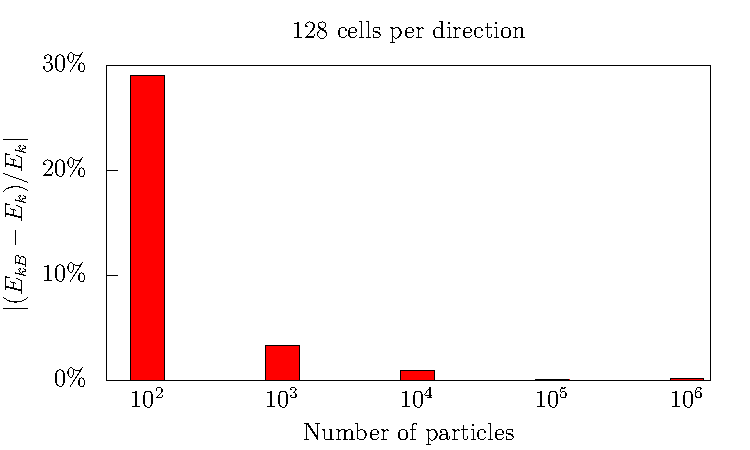
\includegraphics[width=\textwidth]{./../Simulationsergebnisse/variationPartikelAnzahl//128/kineticEnergy_numberOfParticles.pdf}
	\caption{Results for initializing different numbers of particles}
	\label{kineticEnergy_numberOfParticles}
\end{figure}
The normalized difference in turbulent kinetic Energy shows in this one-time simulation a correlation between particle number and accuracy in the simulation. Although this was just a single initialization of particles in a flow, it can be stated that simulations using only $10^2$, $10^3$ or even up to $10^4$ particles are not accurate enough for technical or scientific use of the data. One-time simulations in other grid sizes show similar results.
\pagebreak
\section{Conclusion and outlook}
In this work two sets of simulations were carried out to evaluate a method for lowering computational effort and to find a limit of particles at which a simulation becomes inaccurate. 
\newline
To achieve this goals, first the mathematical basics for understanding particle-free and particle-laden flows were introduced. The reader achieved knowledge about the Navier-Stokes equations and their enhancement for computing interactions between fluid and particles. In the following the reader got information about the numerical basics and methods for simulating such complicated phenomena. 
\newline
The results presented in this work show, that for a sufficiently exact simulation, particle clustering has to be treated with caution. Depending on the application maybe small numbers of clustered particles could be used, but the savings in computing time would not balance out the loss in accuracy. This is the case in particular high numbers of clustered particles at which the results get highly inaccurate. Maybe investigations on smaller numbers of clustered particles could follow, the space between 2 and 10 could be closed by simulations in the future to determine the real border for inaccurate results. 
\newline
Further investigation is needed regarding the second set of simulation, in which the goal was to find out which number of particles is necessary to get accurate results for the turbulent kinetic energy of the particles. The deviation of the averaged kinetic energy of the particles and the fluid should be zero. This difference converges to zero with high numbers of particles. The distribution of the experiment`s outcomes should match the well-known normal distribution, which leads to analyzing the standard deviation. Concluding, further simulations should be carried out until a sufficient standard deviation can be computed, from which an assumption about the accuracy of the initialization could be made.
\subsection*{Acknowledgements}
This work was supervised by Konstantin Fr\"ohlich, we would like to express our gratitude. Thank you for the chance of learning about turbulent flows and simulations, the advice and the deep insights in scientific work. We also want to appreciate the chance of writing this work at the Institute of Aerodynamics of the RWTH Aachen University.
\pagebreak
\section{References}
\nocite{*} %erm�glicht, dass auch Literatur, welche nicht zitiert wurde in der Bibliography auftaucht
\bibliography{Projektarbeit} %ruft die Bibliography-Datei auf
\bibliographystyle{plain} %setzt den Zitierstil
\pagebreak
\end{document}
